\chapter{树莓派}
\section{树莓派简介}
Raspberry Pi,中文名为“树莓派”,简写为 RPi,是一款基于Debian GNU/Linux操作系统的微型计算机,由英国树莓派基金会开发并推出。它小巧、便携,却有着强大的计算能力和丰富的扩展接口,广泛应用于物联网、嵌入式系统、教育、娱乐等领域。
\par
我们使用的是树莓派4B,内存8G。价格较为昂贵且并无多余设备,因此一定小心使用,避免损坏。
\begin{figure}[h]
	\centering
	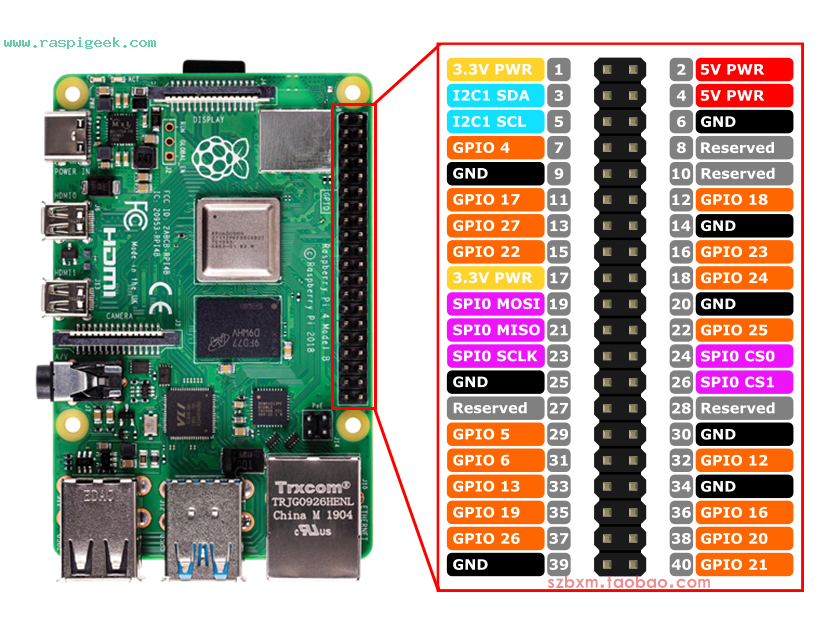
\includegraphics[width=\defaultimagewidth]{树莓派4B引脚.png}
	\caption{树莓派4B引脚}
	\label{fig:example}
\end{figure}
\par
散热用风扇使用5V供电,因此可以将其红黑线分别插于4、6号引脚。,如下图所示
\begin{figure}[H]
	\centering
	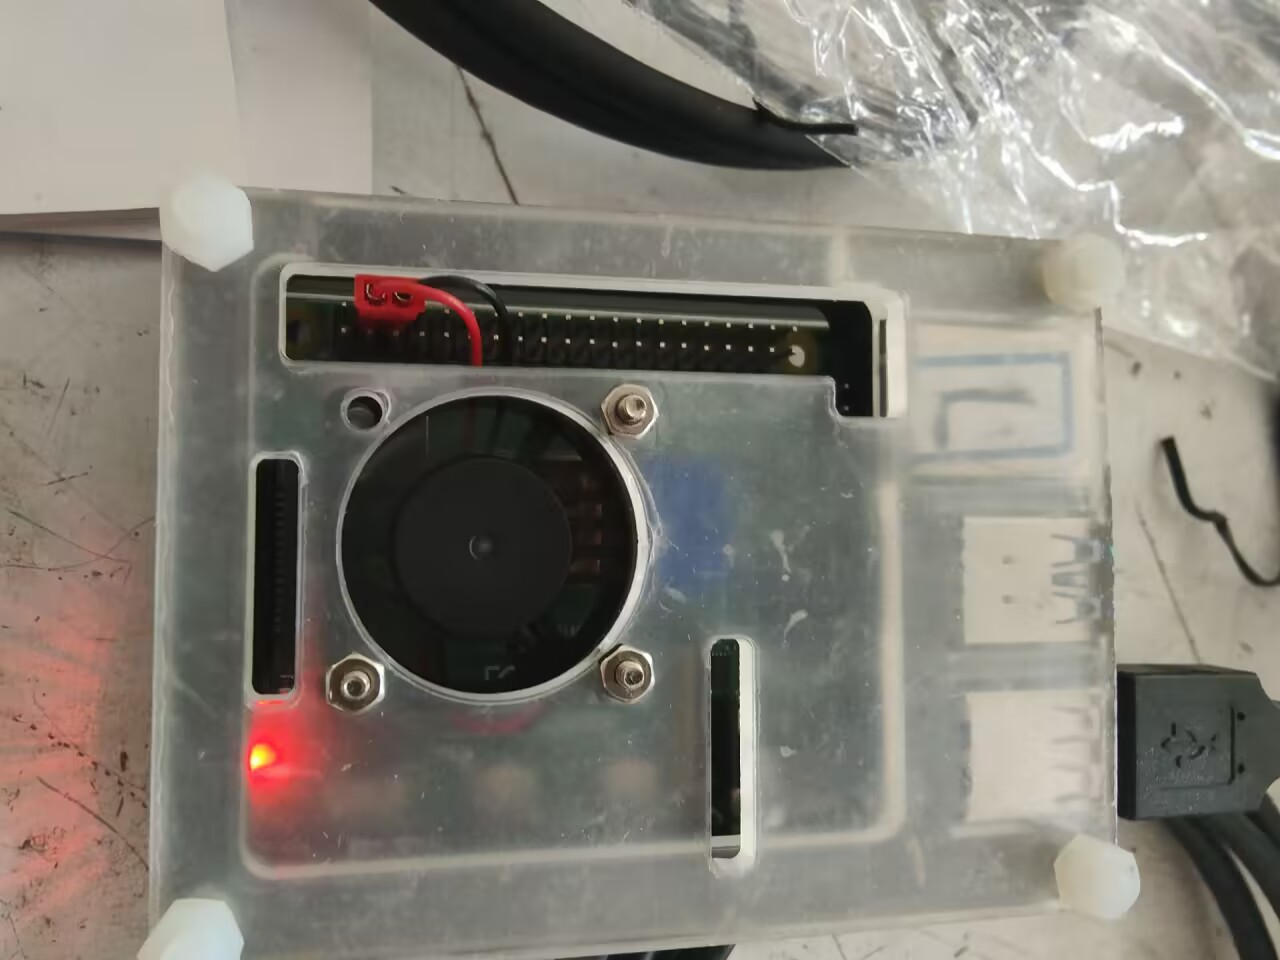
\includegraphics[width=\textwidth]{风扇.jpg}
	\caption{风扇插接}
	\label{fig:example}
\end{figure}
\section{树莓派与显示屏}
接线方式如图所示,注意USB线的另一端接到显示屏的TOUCH口,意即触屏。
\begin{figure}[H]
	\centering
	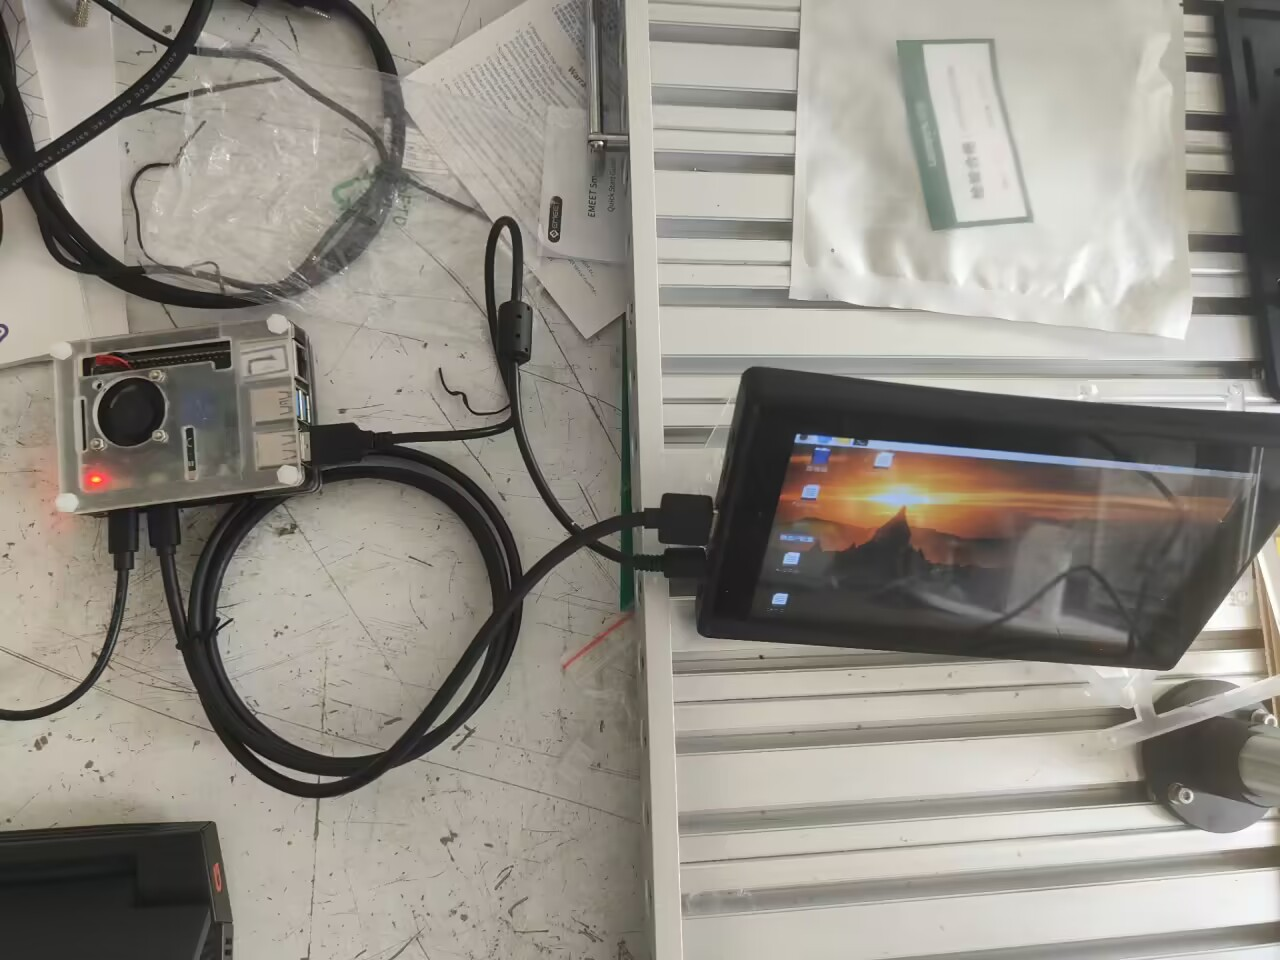
\includegraphics[width=\textwidth]{显示器.jpg}
	\caption{树莓派连接显示屏}
	\label{fig:example}
\end{figure}

\section{树莓派连接Wifi}
接下来配置树莓派连接Wifi。树莓派不支持5GWifi,只支持2.4G,推荐使用个人热点。
\par
首先在终端中输入以下命令:
\begin{lstlisting}[style=bashstyle]
sudo nano /etc/wpa_supplicant/wpa_supplicant.conf
\end{lstlisting}
\par
wpa\_supplicant.conf 这个文件是 Linux 系统中用于配置无线网络接口的配置文件。这个文件被 wpa\_supplicant 程序使用,后者是一个用于管理网络安全(尤其是 WPA 和 WPA2,即 Wi-Fi 保护访问)的客户端程序。
输入命令并回车后能看到下图所示:
\begin{figure}[H]
	\centering
	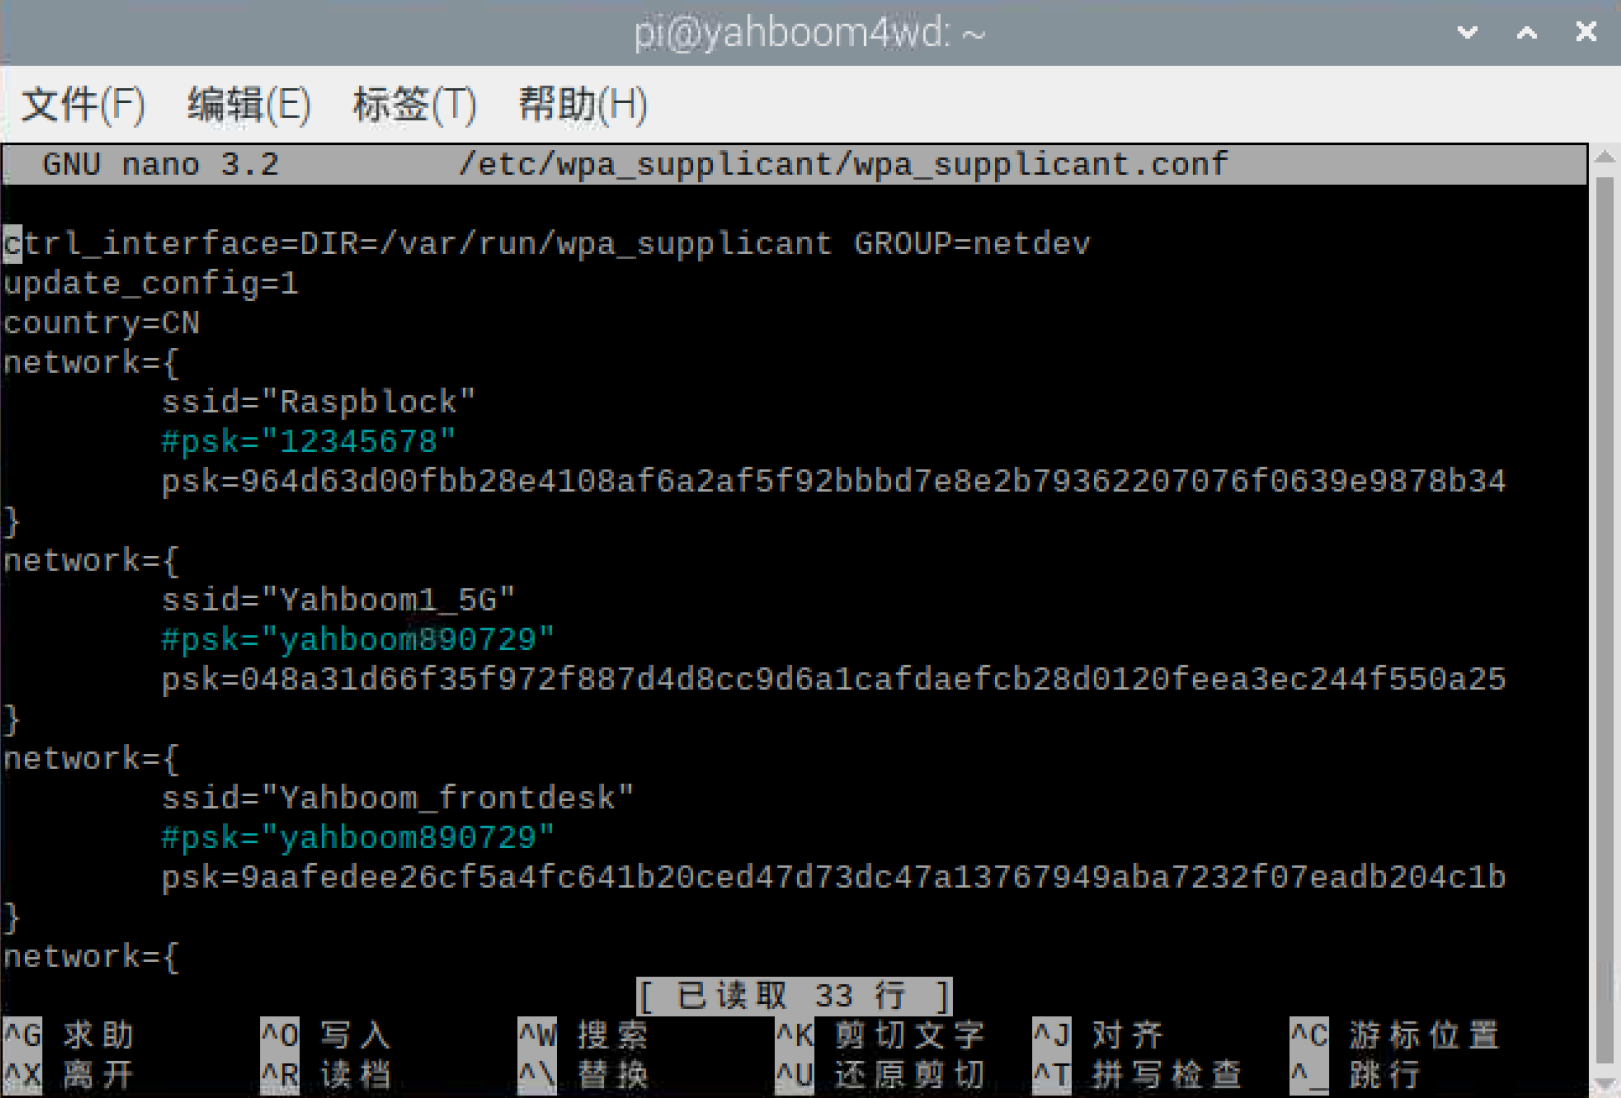
\includegraphics[width=\textwidth]{wpa.png}
	\caption{无线网络配置文件}
	\label{fig:example}
\end{figure}
文件开始的地方应当有country=CN,它的作用是设置无线操作的国家代码为中国China。
\par
这个文件的主要格式为
\begin{lstlisting}[style=bashstyle]
	network={
		ssid="你的网络名称"
		psk="你的密码"
	}
\end{lstlisting}
\par
参照上面的在文件最后加上即可。每一个network字典就代表着去尝试连接的Wifi。按快捷键Ctrl+S表示保存,Ctrl+X表示退出。
\par
接下来修改DHCP配置文件,以设置WLAN静态IP。在终端中输入
\begin{lstlisting}[style=bashstyle]
	sudo nano /etc/dhcpcd.conf
\end{lstlisting}
效果如下图所示:
\begin{figure}[H]
	\centering
	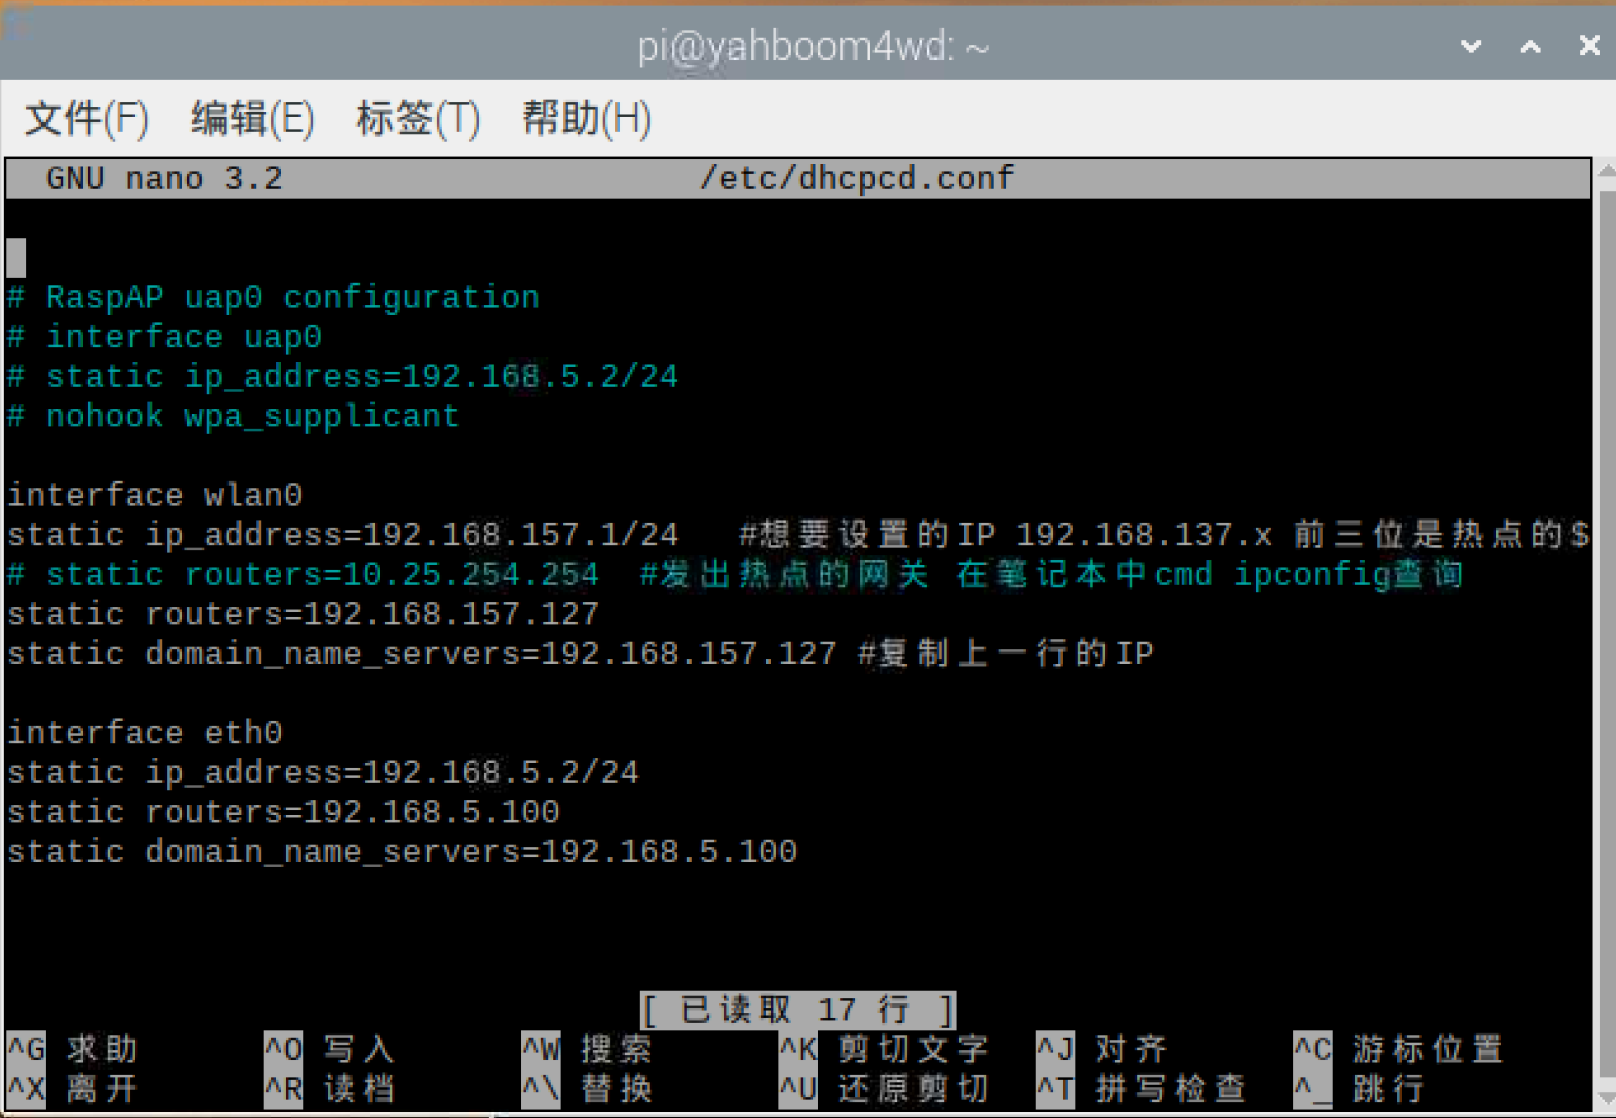
\includegraphics[width=\textwidth]{dhcpcd.png}
	\caption{DHCP配置文件}
	\label{fig:example}
\end{figure}
\par
在其中写入
\begin{lstlisting}[style=configstyle]
	interface wlan0
	static ip_address=192.168.157.1/24	# 静态IP
	static routers=192.168.157.127	# 网关
	static domain_name_servers=192.168.157.127 # DNS
\end{lstlisting}
值得注意的是,参数并非与上面的示例相同。首先用笔记本电脑连接Wifi,然后在电脑的终端中输入
\begin{lstlisting}[style=bashstyle]
	ipconfig
\end{lstlisting}
\par
找到无线局域网适配器WLAN一项:
\begin{figure}[H]
	\centering
	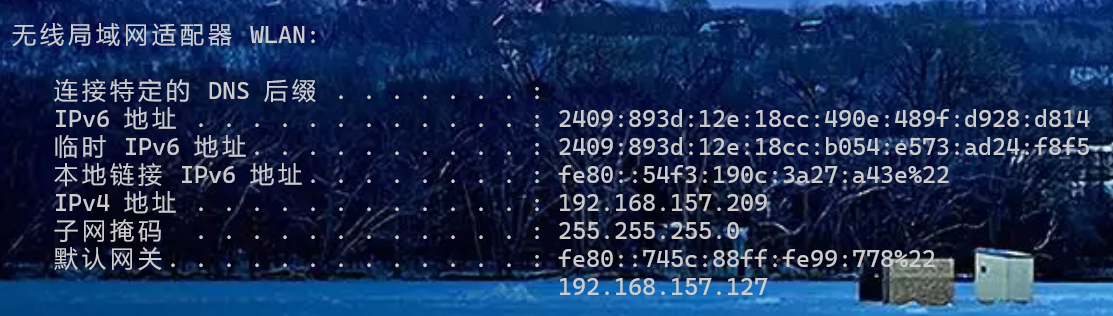
\includegraphics[width=\textwidth]{无线网适配器WLAN.png}
	\caption{无线网适配器WLAN}
	\label{fig:example}
\end{figure}
可以看到图中的IPv4地址和默认网关(下面那行,意思是IPv4的),这两个分别对应着DHCP配置文件中的ip\_address和routers。此外, domain\_name\_servers可以与routers写作一个。
\par
保存并退出即可。
\par
接下来重启树莓派,应当可以连接到Wifi了。

\section{Python开发环境}
树莓派中已经安装好了opencv-python,但可能有依赖需要更新。\\
打开终端,输入
\begin{lstlisting}[style=bashstyle]
	sudo apt-get update
	sudo apt install libxrender1 libvpx5 libxi6 libxcb-render0 libtwolame0 libwebpmux3 libvorbisenc2 libgraphite2-3 libva-x11-2 libwayland-egl1 libgme0 libmp3lame0 libcairo-gobject2 libspeex1 libavcodec58 libswresample3 libwebp6 libcroco3 libdrm2 libxvidcore4 libtheora0 libxfixes3 libvdpau1 libwayland-client0 libjbig0 libcodec2-0.8.1 libharfbuzz0b libatlas3-base libgdk-pixbuf2.0-0 libssh-gcrypt-4 libmpg123-0 libaom0 libogg0 libpangocairo-1.0-0 libxcb-shm0 libbluray2 libopenmpt0 libpangoft2-1.0-0 libatspi2.0-0 libwayland-cursor0 libxrandr2 libxinerama1 libxcomposite1 libgtk-3-0 libxkbcommon0 libva-drm2 libgsm1 librsvg2-2 libopenjp2-7 libxdamage1 libx265-165 libpixman-1-0 libswscale5 libavutil56 libcairo2 libx264-155 libatk1.0-0 libpango-1.0-0 libthai0 libfontconfig1 libxcursor1 libavformat58 libopus0 libdatrie1 libvorbis0a libsoxr0 libva2 libatk-bridge2.0-0 libzvbi0 libshine3 libvorbisfile3 libepoxy0 libchromaprint1 libwavpack1 libtiff5 libgfortran5 libsnappy1v5
\end{lstlisting}
即可安装上述依赖。
\par
安装完成后,在终端中输入
\begin{lstlisting}[style=bashstyle]
	python3
\end{lstlisting}
即可进入python环境。进入后输入
\begin{lstlisting}[style=pythonstyle]
	import cv2
\end{lstlisting}
\par
如果没有出现错误,说明opencv可以正常使用。
\begin{figure}[H]
	\centering
	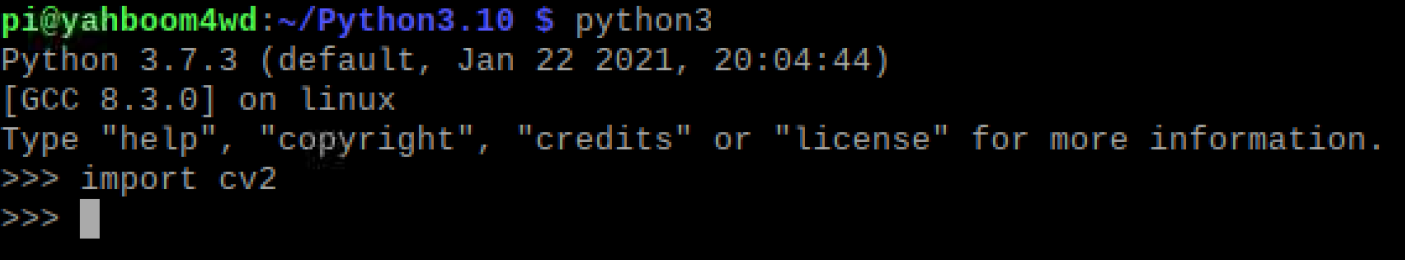
\includegraphics[width=\textwidth]{测试opencv.png}
	\caption{opencv可以正常使用}
	\label{fig:example}
\end{figure}
\par
此外,为保证工程的条理性,建议在家目录(/home/pi或者/home/admin等)下新建一个有标识性的文件夹,用以存放个人文件。例如:
\begin{figure}[H]
	\centering
	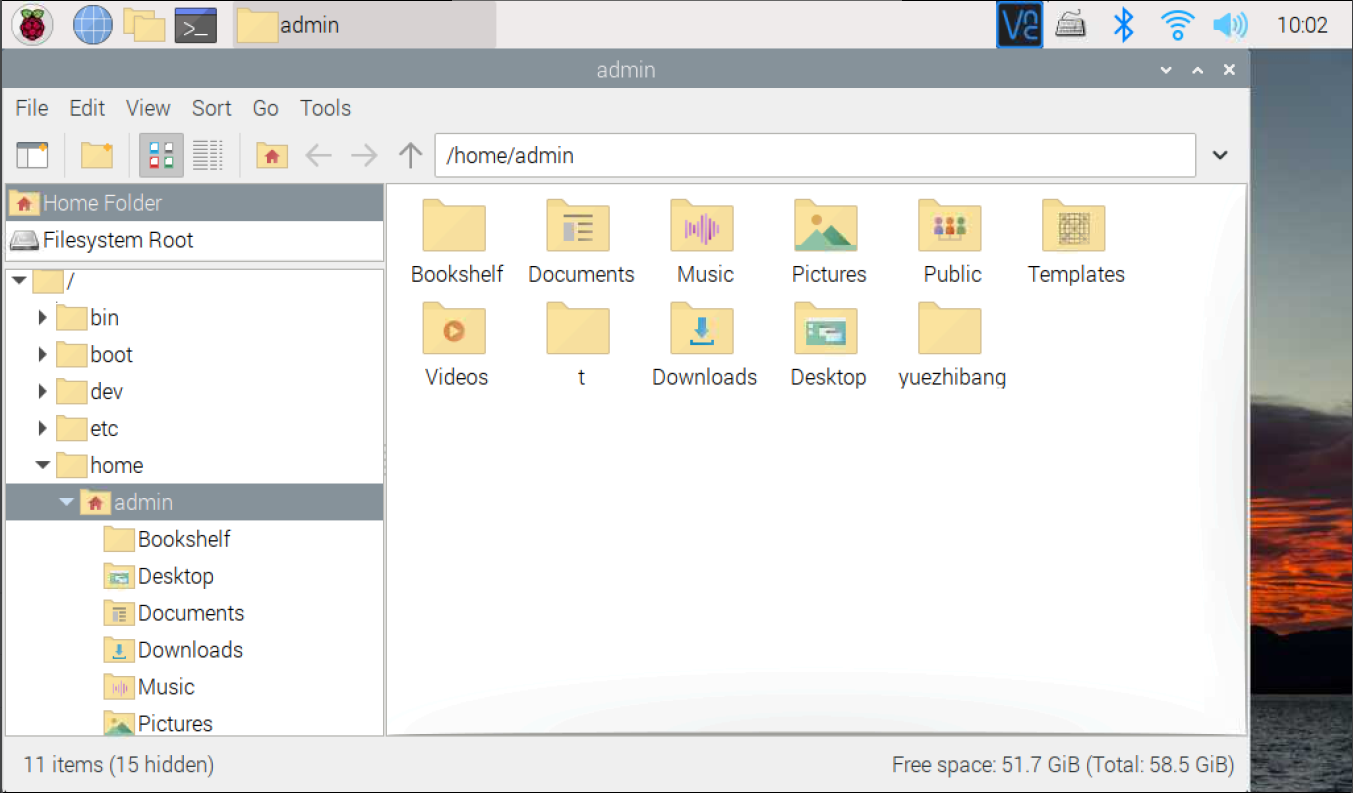
\includegraphics[width=\textwidth]{家目录.png}
	\caption{家目录}
	\label{fig:example}
\end{figure}
\section{以太网静态IP设置}
为了通过网线连接机械臂,树莓派的以太网IP应当是静态的。
\par
设置方法与连接Wifi相似,仍然是编辑DHCP配置文件:
\begin{lstlisting}[style=bashstyle]
	sudo nano /etc/dhcpcd.conf
\end{lstlisting}
在其中添加以下内容
\begin{lstlisting}[style=configstyle]
	interface eth0
	static ip_address=192.168.5.2/24
	static routers=192.168.5.1
	static domain_name_servers=192.168.5.1
\end{lstlisting}
\par
上面这段代码是以太网静态IP设置,eth0指定为网线连接设置。这里设置静态IP为192.168.5.2/24,意思是IP为192.168.5.2,24代表子网掩码为255.255.255.0,此外设置路由网关为192.168.5.1。
\par
这样设置,是由Dobot的通讯设置所决定,如下图:
\begin{figure}[H]
	\centering
	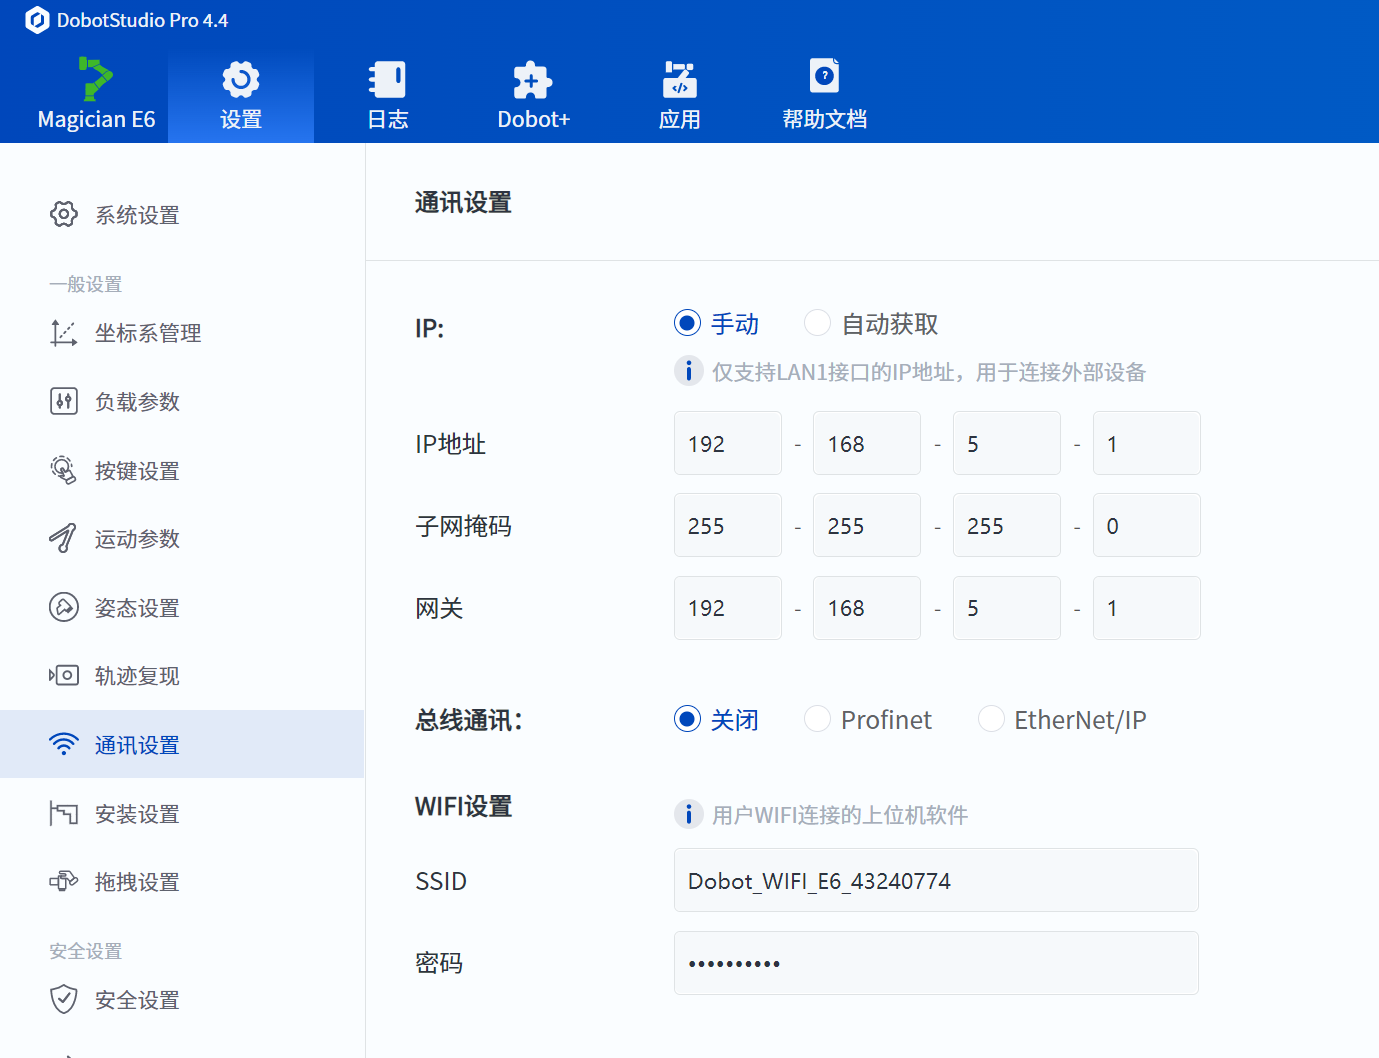
\includegraphics[width=\textwidth]{通讯设置.png}
	\caption{通讯设置}
	\label{fig:example}
\end{figure}
建议如上图配置。
\par
保存并退出,重启树莓派即可。

\section{树莓派外接摄像头}
将我们的摄像头像显示屏一样连接到树莓派上,在终端中输入
\begin{lstlisting}[style=bashstyle]
	lsusb
\end{lstlisting}
看到下图所示:
\begin{figure}[H]
	\centering
	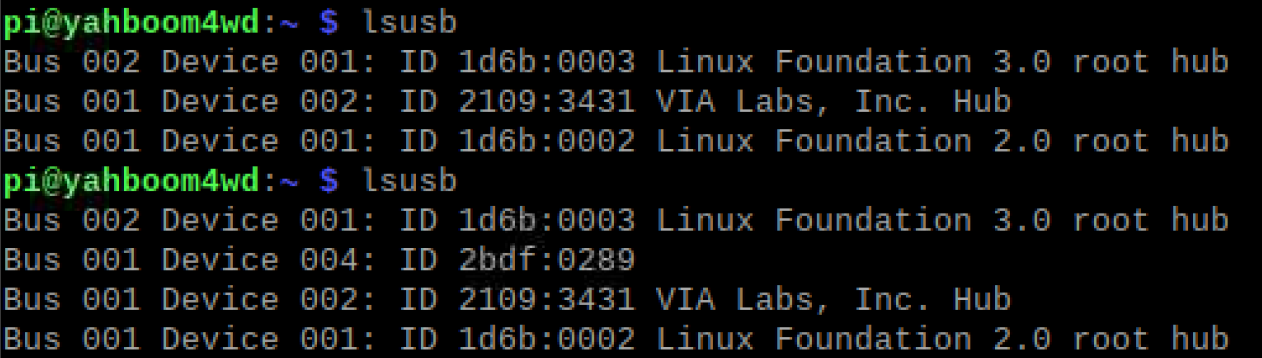
\includegraphics[width=\textwidth]{lsusb.png}
	\caption{USB设备}
	\label{fig:example}
\end{figure}
本来是三个,插上摄像头之后再输入该命令,可以观察到多出来了一个。多出来的这个就是摄像头。
\par
此外,输入
\begin{lstlisting}[style=bashstyle]
	ls -l /dev/video*
\end{lstlisting}
可以显示所有视频设备,观察时间一栏,如果有时间新近的,说明就是刚刚连接上的摄像头。
\par
接下来测试一下效果。比如说可以新建一个python文件camera\_test.py,内容如下:
\begin{lstlisting}[style=pythonstyle]
import cv2
import numpy as np

# 鼠标回调函数
def mouse_click(event, x, y, flags, param):
	if event == cv2.EVENT_LBUTTONDOWN:
	# 当鼠标左键被按下时打印坐标信息
		print(f'Mouse Position: (X: {x}, Y: {y})')
# 开启摄像头
cap = cv2.VideoCapture(0)
if not cap.isOpened():
	print("Cannot open camera")
	exit()
cv2.namedWindow('Frame')
cv2.setMouseCallback('Frame', mouse_click)
while True:
	ret, frame = cap.read()
	if not ret:
		print("Can't receive frame (stream end?). Exiting ...")
		break	
	cv2.imshow('Frame', frame)
	# 按 'q' 键退出循环
	if cv2.waitKey(1) & 0xFF == ord('q'):
		break
# 释放摄像头资源并关闭窗口
cap.release()
cv2.destroyAllWindows()
\end{lstlisting}
\par
运行程序后,能有显示画面的窗口弹出,说明摄像头和opencv可以正常使用。
\begin{figure}[H]
	\centering
	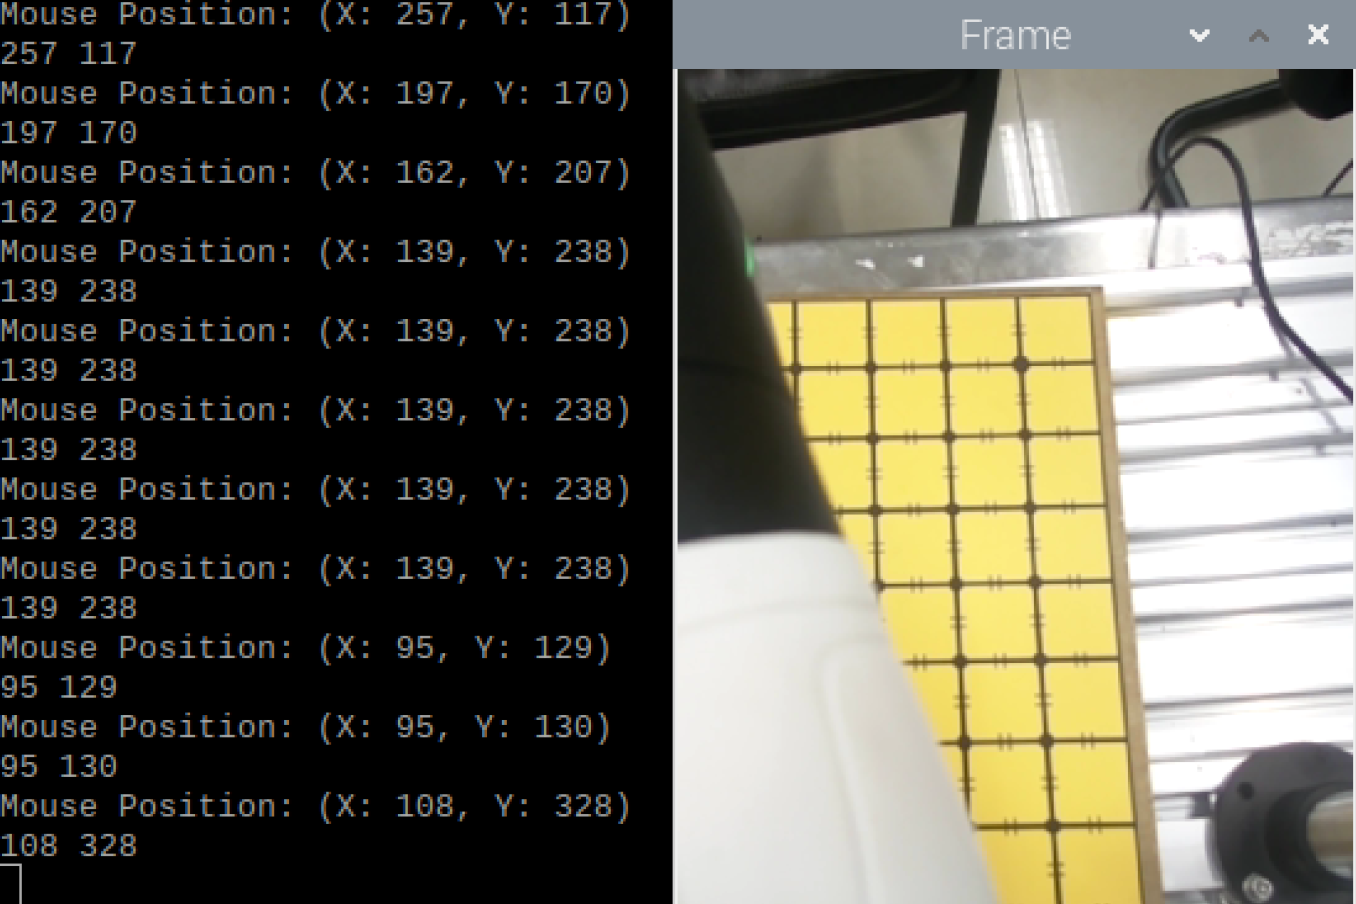
\includegraphics[width=0.8\textwidth]{测试摄像头.png}
	\caption{摄像头和opencv可以正常使用}
	\label{fig:example}
\end{figure}

\section{远程桌面连接树莓派}
远程连接的前提是已经确定了树莓派的IP地址,前面我们让树莓派连接了Wifi,并且设置静态IP为192.168.157.1,只要我们的电脑与它处在同一个无线网络下,就可以在电脑上远程连接了。
\par
以VNC为例(VNC是一款强大的远程控制软件):
\par 
首先,应确保树莓派开启了VNC权限。操作步骤如下:
\begin{figure}[H]
	\centering
	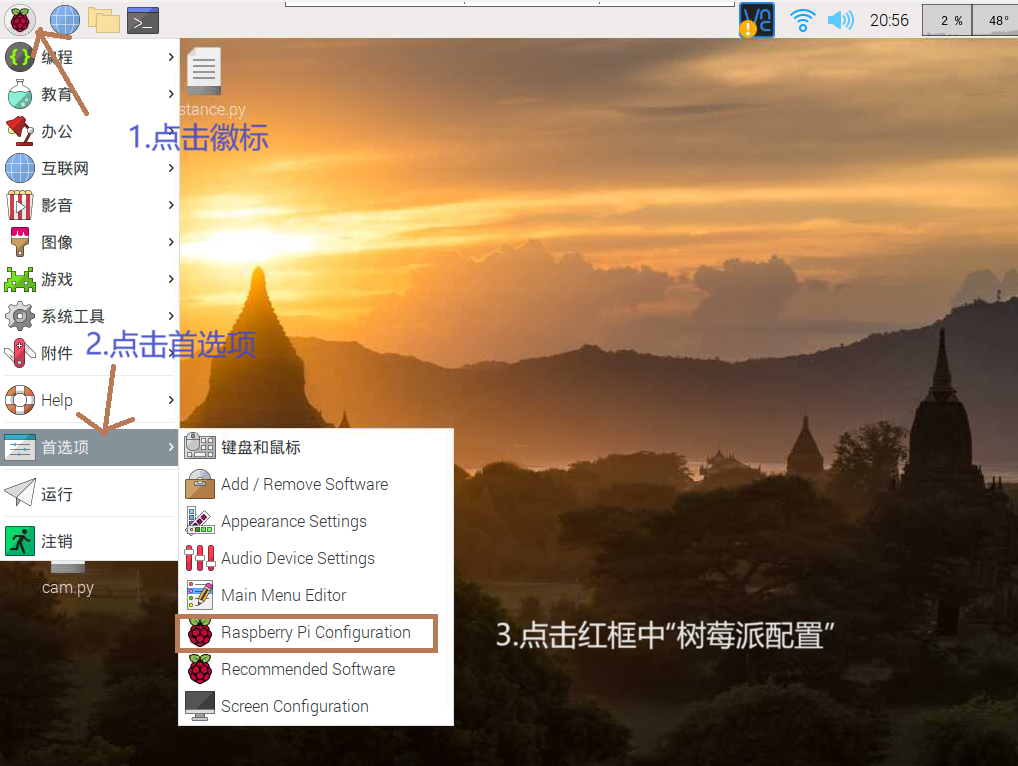
\includegraphics[width=\textwidth]{树莓派设置.png}
	\caption{打开树莓派设置}
	\label{fig:example}
\end{figure}
点击左上角徽标,点击首选项,点击Raspberry Pi Configuration,进入设置界面。
\par 
点击Interfaces,把VNC一项设定为Enable,如下图。
\begin{figure}[H]
	\centering
	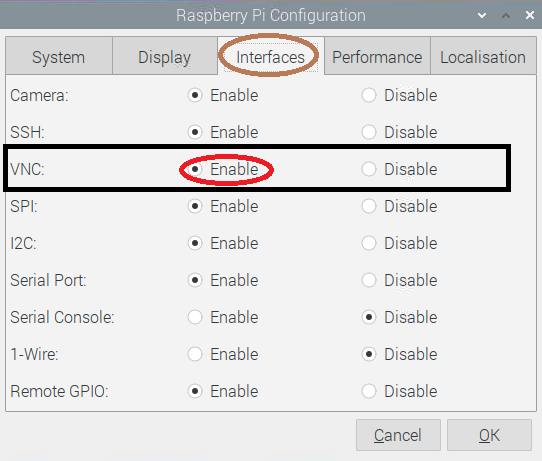
\includegraphics[width=\textwidth]{VNC权限.png}
	\caption{打开VNC权限}
	\label{fig:example}
\end{figure}
树莓派的VNC权限就打开了。
\par 
然后,在电脑上打开VNC,按下Ctrl+N,打开新建连接界面,如下图:
\begin{figure}[H]
	\centering
	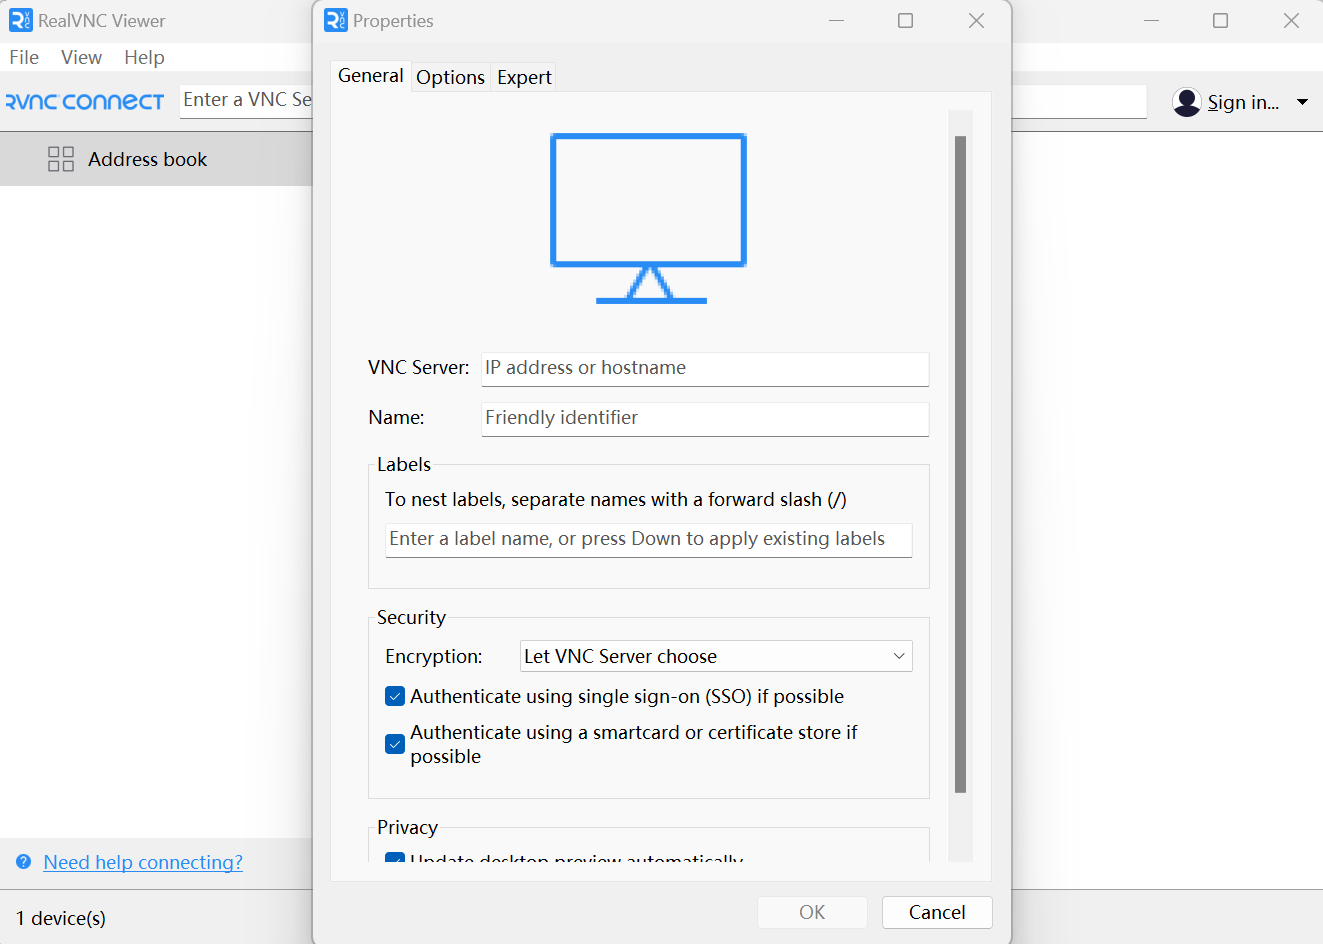
\includegraphics[width=\textwidth]{VNC.png}
	\caption{VNC新建连接}
	\label{fig:example}
\end{figure}
在VNC Server处输入树莓派的IP地址192.168.157.1(参考连接Wifi时设置的IP地址),点击OK即可连接。
初次连接时可能会会弹出如下的弹窗,点击Continue即可。
\begin{figure}[H]
	\centering
	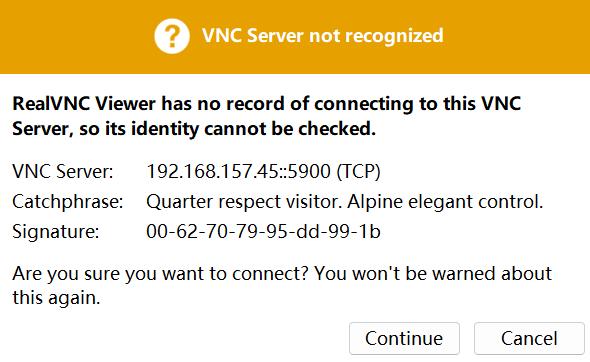
\includegraphics[width=\textwidth]{继续.png}
	\caption{初次连接时}
	\label{fig:example}
\end{figure}
\par 
之后进入登录弹窗,在表单中输入用户名pi(或者admin),密码raspberry(这是树莓派的默认密码),点击OK即可连接,如下图所示。
\begin{figure}[H]
	\centering
	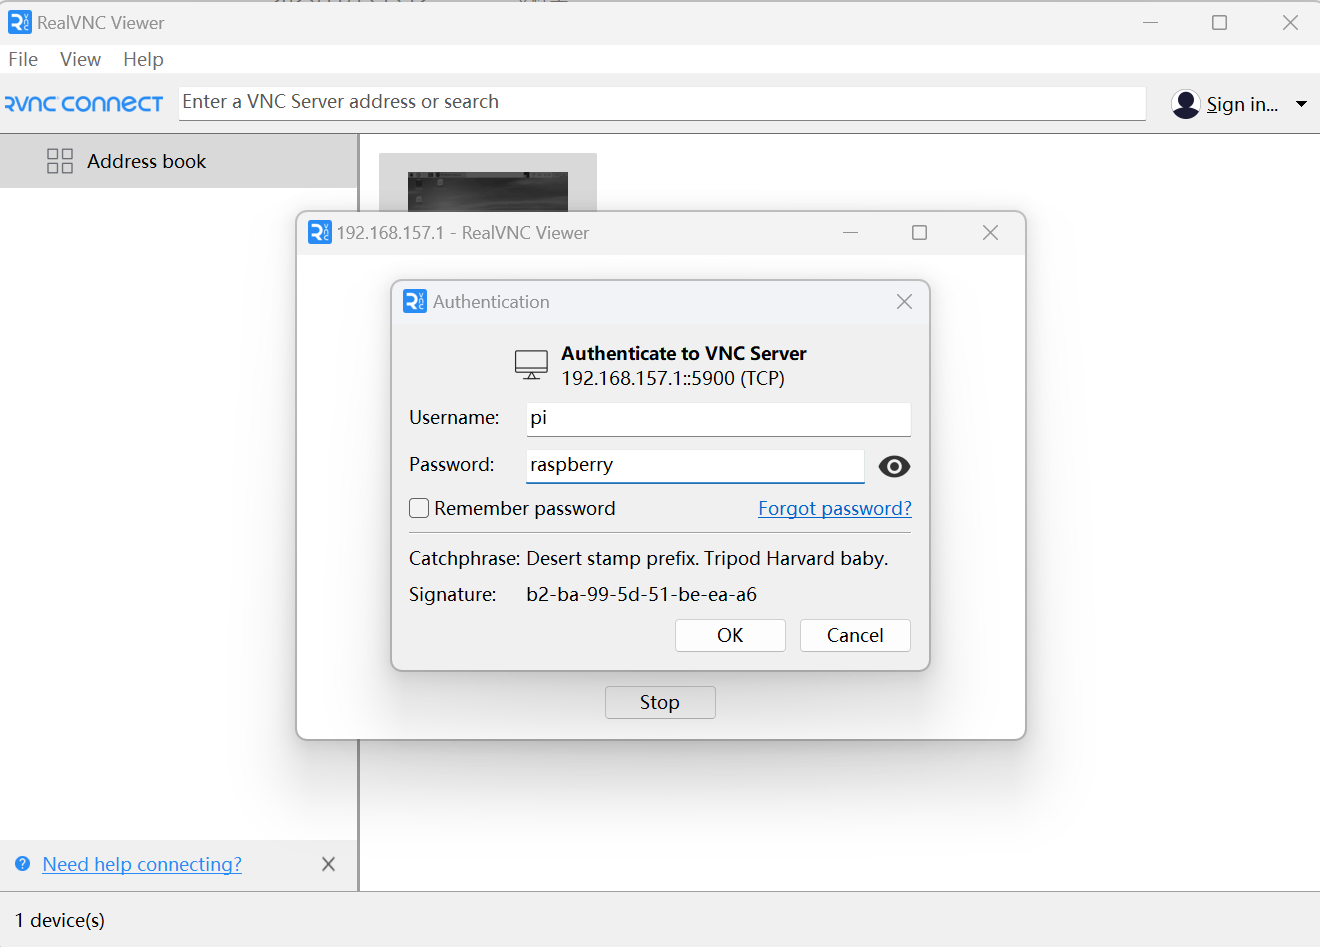
\includegraphics[width=\textwidth]{连接树莓派.png}
	\caption{连接树莓派}
	\label{fig:example}
\end{figure}

\section{与树莓派的文件传输}
在树莓派中编写代码比较困难,因此我们可以在个人电脑上编写好代码再传输到树莓派上运行。我们以WinSCP为例。
\par
打开WinSCP,点击“新建会话”,输入主机(即无线网卡的IP地址,也即连接Wifi时设置的IP地址)、用户名、密码,点击登录,就可以建立起连接,如下图所示。
\par 
主机、用户名、密码其实都与远程桌面连接时使用的一致。
\par 
初次连接时,可能会出现警告弹窗,点击“是”或“否”均可。
\begin{figure}[H]
	\centering
	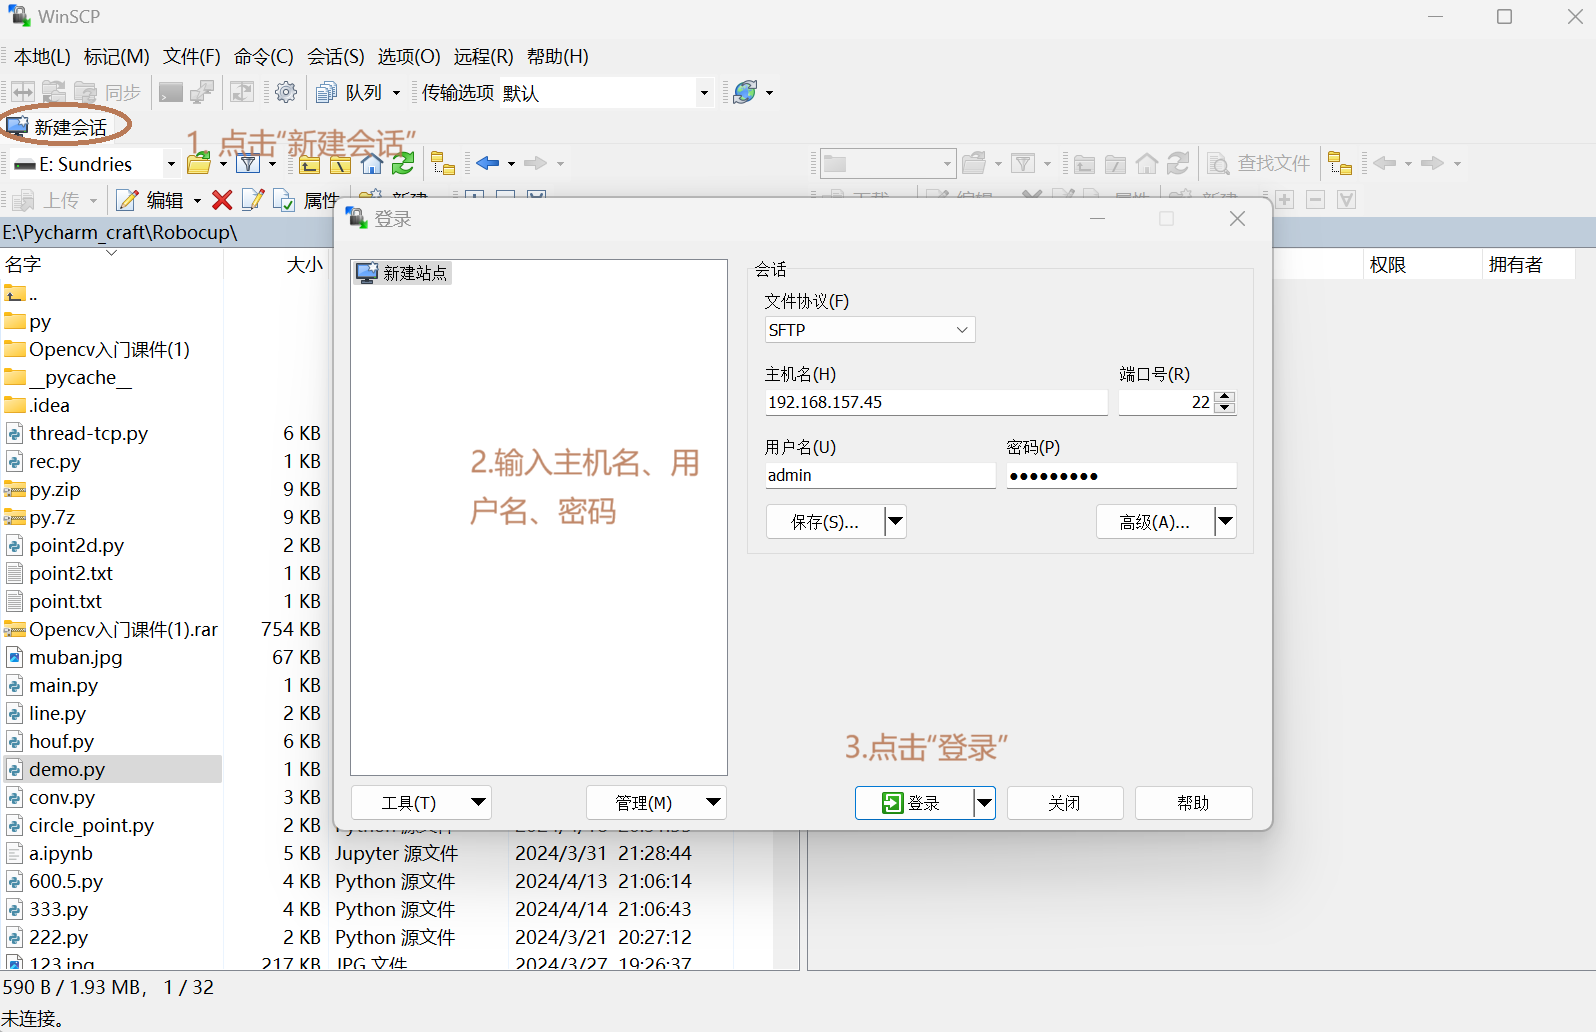
\includegraphics[width=\textwidth]{WinSCP.png}
	\caption{WinSCP连接树莓派}
	\label{fig:example}
\end{figure}
\begin{figure}[H]
	\centering
	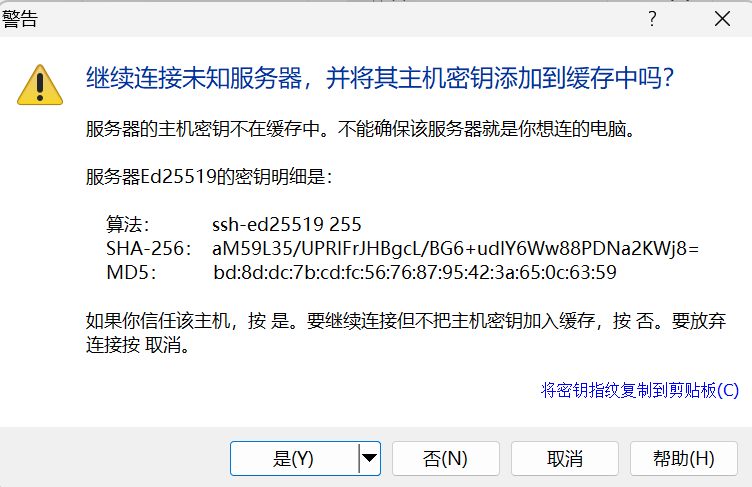
\includegraphics[width=\textwidth]{主机密钥.png}
	\caption{警告}
	\label{fig:example}
\end{figure}
连接成功之后,观察到左栏即为本机,右栏为树莓派,拖拽文件即可传输。
\begin{figure}[H]
	\centering
	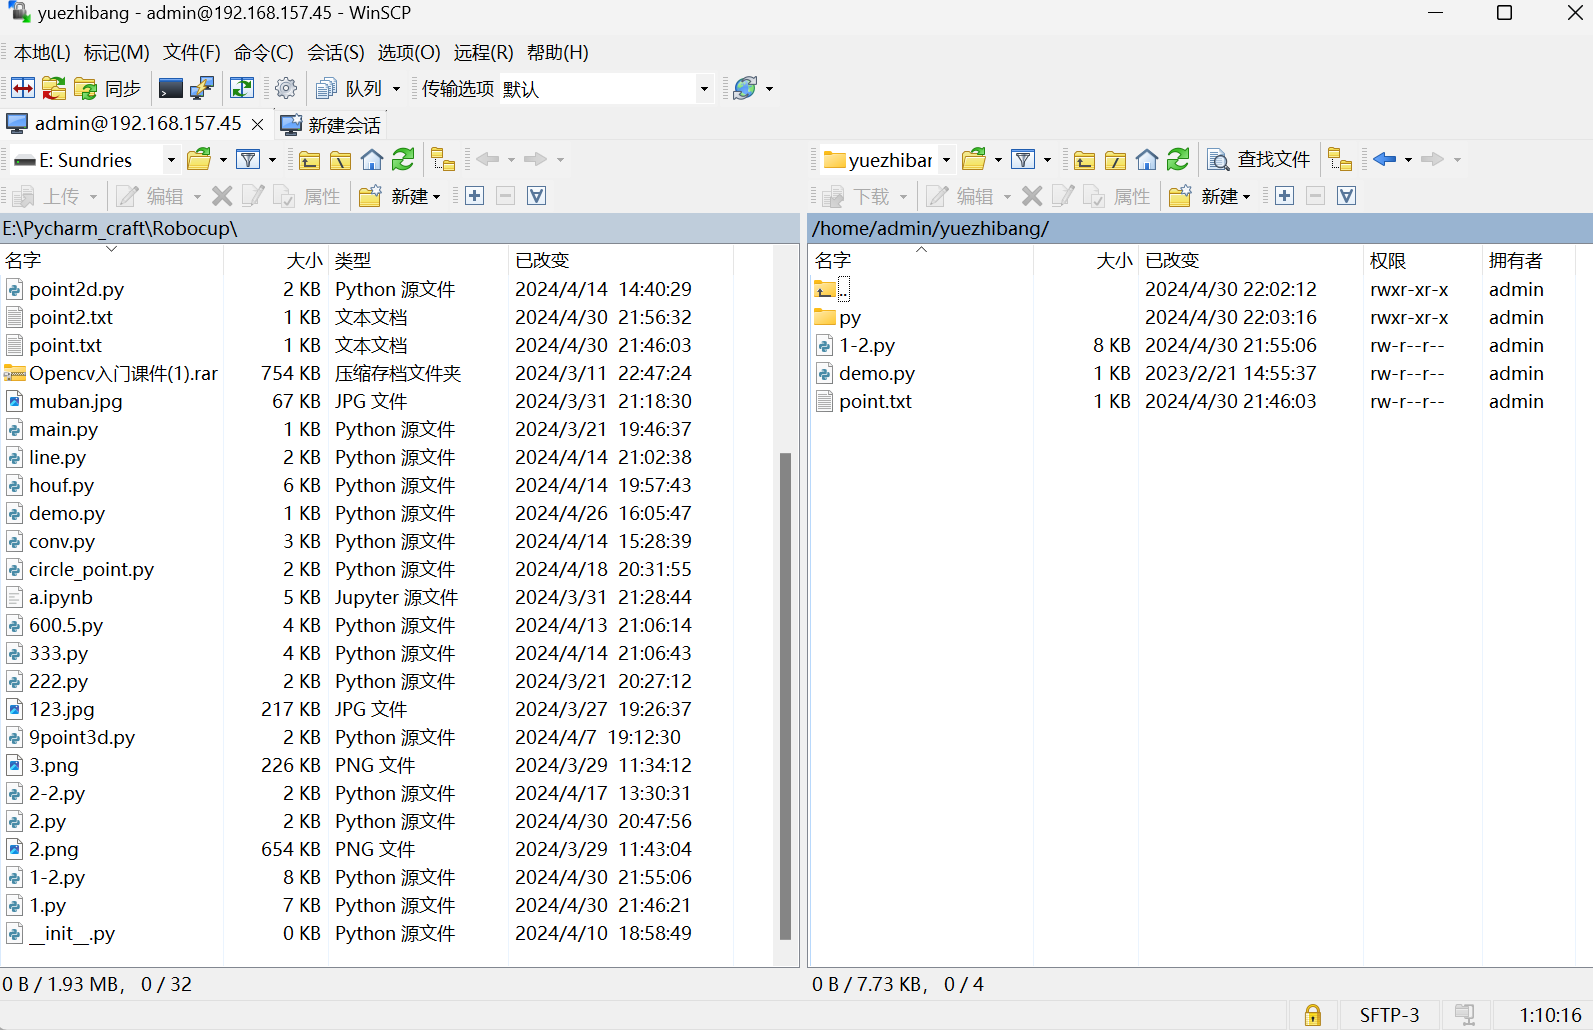
\includegraphics[width=\textwidth]{传输文件.png}
	\caption{传输文件}
	\label{fig:example}
\end{figure}